\mode<all>
% Incluyo los paquetes necesarios.
% para no tener problemas con acentos etc.
\usepackage[utf8]{inputenc}
% en español
\usepackage[spanish]{babel}
%matemática
\usepackage{amsmath}
% este no se si hace falta pero por las dudas
\usepackage{graphicx}
% para incluir peliculas
\usepackage{multimedia}
% para usar segunda pantalla
\usepackage{pgfpages}
\usepackage{pgf}
% para hacer dibujitos
\usepackage{tikz}
\usetikzlibrary[automata,calc,arrows,decorations.pathmorphing,backgrounds,shapes,
patterns,positioning,fit,petri,overlay-beamer-styles]
\tikzstyle{every picture}+=[remember picture]
%recuadros sencillos
%\usepackage{tcolorbox}
% enumeradores intercambiables
\usepackage{enumerate}
% para subtitulos en figuras
\usepackage{subcaption}
%listings for code input
\usepackage{listings}
%verbatim input from file!
\usepackage{verbatim}
\usepackage{fancyvrb}
% para modificar los encabezados y pies de página.
%\usepackage{fancyhdr}
%\pagestyle{fancy}
\usepackage{standalone}

\definecolor{codegreen}{rgb}{0,0.6,0}
\definecolor{codegray}{rgb}{0.5,0.5,0.5}
\definecolor{codepurple}{rgb}{0.58,0,0.82}
%\definecolor{backcolour}{rgb}{0.95,0.95,0.0.1}

\lstset{
    basicstyle=\fontsize{8}{10}\selectfont\ttfamily, 
    backgroundcolor=\color{Beige},   
    frame=lines,
    commentstyle=\color{codegreen},
    keywordstyle=\color{magenta},
    numberstyle=\tiny\color{codegray},
    stringstyle=\color{codepurple},
    breakatwhitespace=false,         
    breaklines=true,                 
    captionpos=b,                    
    keepspaces=true,                 
    numbers=left,                    
    numbersep=5pt,                  
    showspaces=false,                
    showstringspaces=false,
    showtabs=false,                  
    tabsize=4
}



%\mode<presentation>{
% para ver las notas con la presentacion.  
%\setbeameroption{hide notes}
%para dejar las notas en la segunda patnalla
%}

% incluyo los beamercolors
%%%%%%%%%% BEAMERCOLORS
% el recuadro para el titulo
\setbeamercolor{title}{fg=white,bg=Purple}
% el recuadro para el subtitulo
\setbeamercolor{subtitle}{fg=white,bg=DarkOliveGreen}
% los títulos de las secciones tienen su colorinche:
\setbeamercolor{sectionbox}{fg=white,bg=Purple}
% cada diapositiva tendrá su color de título.
\setbeamercolor{frametitle}{fg=white,bg=ForestGreen}
% el título de las secciones tienen también su color. 
\setbeamercolor{sectiontitle}{fg=white,bg=violet}

%%%% CUSTOM BEAMERCOLORS
% estos cuadros los defino para ubicar al lector en los temas que se tratan
% son los cuadritos que aparecen arriba del título. 
\setbeamercolor{structure0}{fg=white,bg=gray}
\setbeamercolor{structure1}{fg=black,bg=DarkGray}
\setbeamercolor{structure2}{fg=black,bg=lightgray}
% defino un cuadro para usar en alguna oportunidad, creo que para titulos. 
\setbeamercolor{whitebox}{fg=black,bg=white}
% un cuadro para resaltar
\setbeamercolor{highlight1}{fg=black,bg=Gold}

% beamer colors for headers and etc.
\setbeamercolor{header1}{fg=white,bg=Blue}
\setbeamercolor{header2}{fg=black,bg=Red}
\setbeamercolor{header3}{fg=black,bg=ForestGreen}

%code block
\setbeamercolor{codeblock}{fg=Blue, bg=Beige}
\setbeamerfont{codeblock}{family=\ttfamily,size=\scriptsize}


%incluyo el tema y modificaciones
%%% BEAMER THEME
% el tema 'boxes' es igual al default pero permite definir boxes de estructura 
% a mano. 
\mode<presentation>{
  \usetheme{boxes}
  % los boxes que identifican lo que se esta leyendo
    % box de la izquierda: la materia (subtitulo)
    \addheadbox{structure2}{\quad \tiny \insertshortsubtitle}
  %  box del medio en cabecera, el titulo de la clase
    \addheadbox{structure0}{\quad \tiny  \inserttitle \quad } 
  % box en a la derecha , eltítulo de la sección. 
    \addheadbox{structure1}{\quad \tiny \insertsection}
}
% tema interno y de colores para las diapositivas normales. 
\useinnertheme{rectangles}
\usecolortheme{dove}
% la fuente de las ecuaciones
\usefonttheme[onlymath]{serif}

% entorno codeblock para meter piezas de código.
% el color se definió en BEAMERCOLORS

\newenvironment{codeblock}
{
  \begin{beamercolorbox}{codeblock}
    \usebeamerfont{codeblock}
}
{
  \end{beamercolorbox}
}



% modifico los temas
  \titlegraphic{%
\includegraphics[width=0.25\textwidth]{./PREAMBLE/logo-isabt25.png}
                
\includegraphics[width=0.25\textwidth]{./PREAMBLE/logo-isabato.png}
  		\hfill
		
\includegraphics[width=0.25\textwidth]{./PREAMBLE/ISOLOGOCNEA.png}
		\hfill
  		
\includegraphics[width=0.25\textwidth]{./PREAMBLE/unsam-horizontal.png}}

\mode<presentation>{
\setbeamertemplate{title page}[center]
{
  %
\includegraphics[width=0.25\textwidth]{./PREAMBLE/ISOLOGOCNEA.png}
  \inserttitle
  \insertsubtitle
  \insertauthor
  \insertinstitute
%  \inserttitlegraphic
}
}


% defino el template para las dapositivas con los titulos de las secciones. 
%es una recetita que saqué de algun lado. 
\setbeamertemplate{section page}{
  \begin{beamercolorbox}[ht=5ex,dp=1ex,wd=\paperwidth,center]{sectionbox}
    \begin{centering}
     \usebeamerfont{section  title} \insertsection 
    \end{centering}
  \end{beamercolorbox}
}
\AtBeginSection[]{
  \begin{frame}[plain]
    \begin{center}
    \quad \inserttitle \quad  
    \end{center}
    \sectionpage
  \end{frame}
}

% remover los simbolos de navegacion
% porque sacan espacio 
\mode<presentation>{
\setbeamertemplate{navigation symbols}{}
\setbeamertemplate{footline}[page number]
% me gustan los titulos a la derecha
\setbeamertemplate{frametitle}[default][right]%{
}
\mode<handout>{
 \setbeamertemplate{headline}{}
 \setbeamertemplate{frametitle}{}
 \setbeamertemplate{background}{
   \tikz\node [rectangle,minimum width=0.995\paperwidth,
   minimum height=0.995\paperheight,draw,anchor=south west,
   line width=2pt]  {};
 }
 \setbeamertemplate{footline}{}
}
% aparentemente el siguiente beamertemplate
%se ejecuta en modo artículo. habría que ver
%la forma de sacale probecho. 
% notar que vale solo para las framesque se incluyen 
% directamente en el artículo y no vale para 
% \includeslide.
% \setbeamertemplate{frame begin}
% \setbeamertemplate{frame end}


% no se si es el mejor lugar para definirlo, 
% pero las \includeslides deben quedar fijas al
% tamaño de la página:

%\mode<article>{
%\renewcommand\includeslide[1]{
%  \includeslide[width=\textwidth]{#1}
%}
%}

% defino el template para la diapositiva del título

%%%%%%%%%%%%%%%%%%%%%%%%%%%%%%%%
% Defino la Clase
%%%%%%%%%%%%%%%%%%%%%%%%%%%%%%%%
\subtitle[Modelización 2020]{ Modelización de Propiedades y Procesos 2021 }
\author{Ruben Weht\inst{1,2} \and Mariano Forti\inst{1,3} }
\institute{
%  \inst{1}Instituto de Tecnología Prof. Jorge Sabato
%  \and
  \inst{1}Fisica del Sólido, Edificio TANDAR, \url{weht@cnea.gov.ar},
  interno 7104
  \and
  \inst{2}División Aleaciones Especiales, Edificio 47 (microscopía),
  \url{mforti@cnea.gov.ar}, interno 7832
}

\mode<presentation>{\date{}}

\mode<article>{
  \date{
    \small
%  \textsuperscript{1} Instituto de Tecnología Prof. Jorge Sabato\\
  \textsuperscript{1}Fisica del Sólido, Edificio TANDAR, \url{weht@cnea.gov.ar},
  interno 7104 \\
  \textsuperscript{2}División Aleaciones Especiales, Edificio 47 (microscopía),
  \url{mforti@cnea.gov.ar}, interno 7832
}

%defino los encabezados y pies de págna para
% dodo el documento en función de la materia y la
% clase.
%\fancyhead[L]{\tiny Modelización de Materiales 2019}
%\fancyhead[R]{\tiny \leftmark}
}

\title{
  \mode<article>{
% 
\includegraphics[height=1cm]{./PREAMBLE/logo-isabt25.png}

\includegraphics[height=1cm]{./PREAMBLE/logo-isabato.png}
\hfill

\includegraphics[height=1cm]{./PREAMBLE/ISOLOGOCNEA.png}
\hfill

\includegraphics[height=1cm]{./PREAMBLE/logo-unsam.png}
\\}  Apéndice: Github}
\subject{Apéndice: Github}
\keywords{Python, Modelizacion 2022, Programación}
%linea para fbox
\setlength\fboxsep{0pt}
\setlength\fboxrule{5pt}
% Inicia el documento.
\begin{document}

% Título de la clase. 
\mode<presentation>{
\begin{frame}[plain]
\titlepage
\end{frame}
}

%\mode<article>{
%\maketitle
%}

\begin{frame}<presentation>[label=FrameGithub]
  \frametitle{Github}

  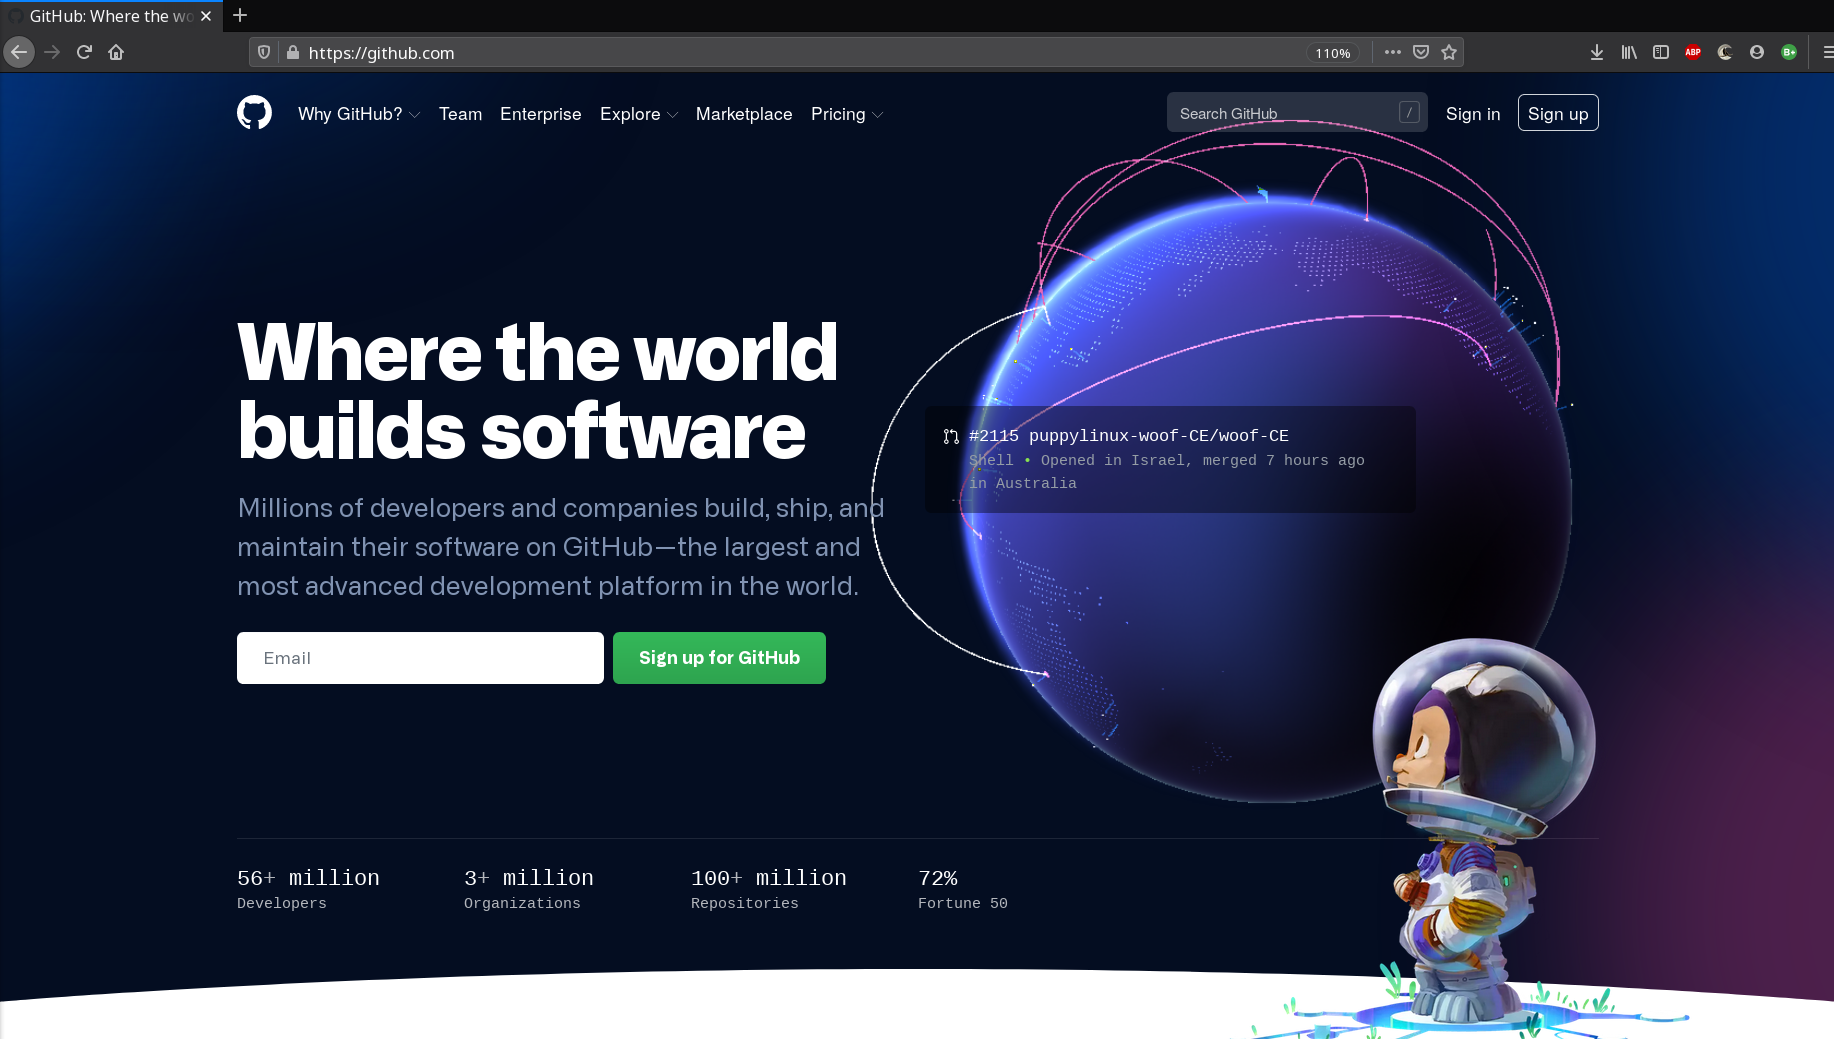
\includegraphics[width=\textwidth]{Screenshots/GithubFrontPag.png}

\end{frame}

\begin{frame}<presentation>[label=FrameRepaso]
  \frametitle{Creamos un usuario}

  \begin{columns}
    \column{0.5\textwidth}

      
\includegraphics[width=\textwidth]{Screenshots/SignUp.png}

      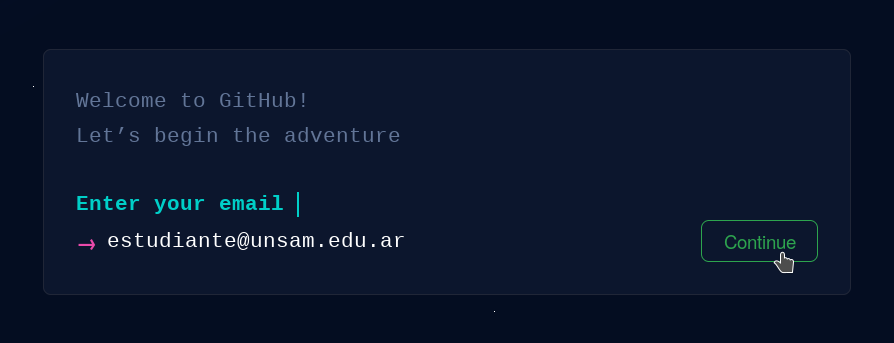
\includegraphics[width=\textwidth]{Screenshots/CrearUsuario.png}

    \column{0.5\textwidth}

      \begin{itemize}
	  \item Sign Up! 
	  \item ingresamos los datos: use un correo electrónico formal!
      \end{itemize}

  \end{columns}

\end{frame}

\begin{frame}<presentation>[label=FrameRepoMateria2022]
  \frametitle{Busque el repositorio de la materia ! }

  \url{https://github.com/Modelizacion-de-Materiales/2022_Ingenieria}

  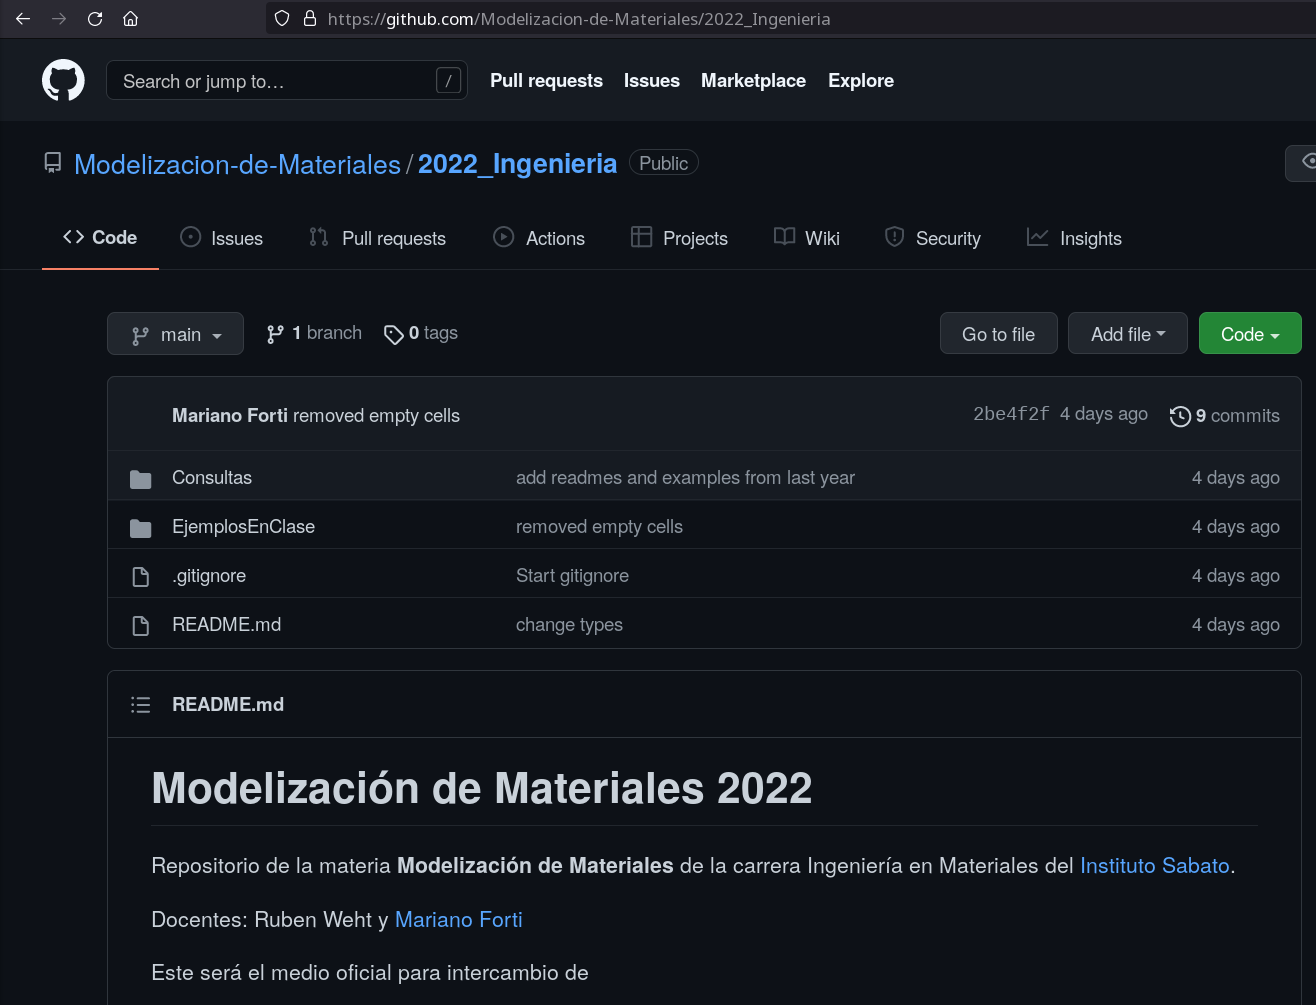
\includegraphics[width=\textwidth]{Screenshots/Repo2022.png}

\end{frame}

\begin{frame}<presentation>[label=FrameMakeFork]
  \frametitle{Haga un Fork (una copia)}

\centering

  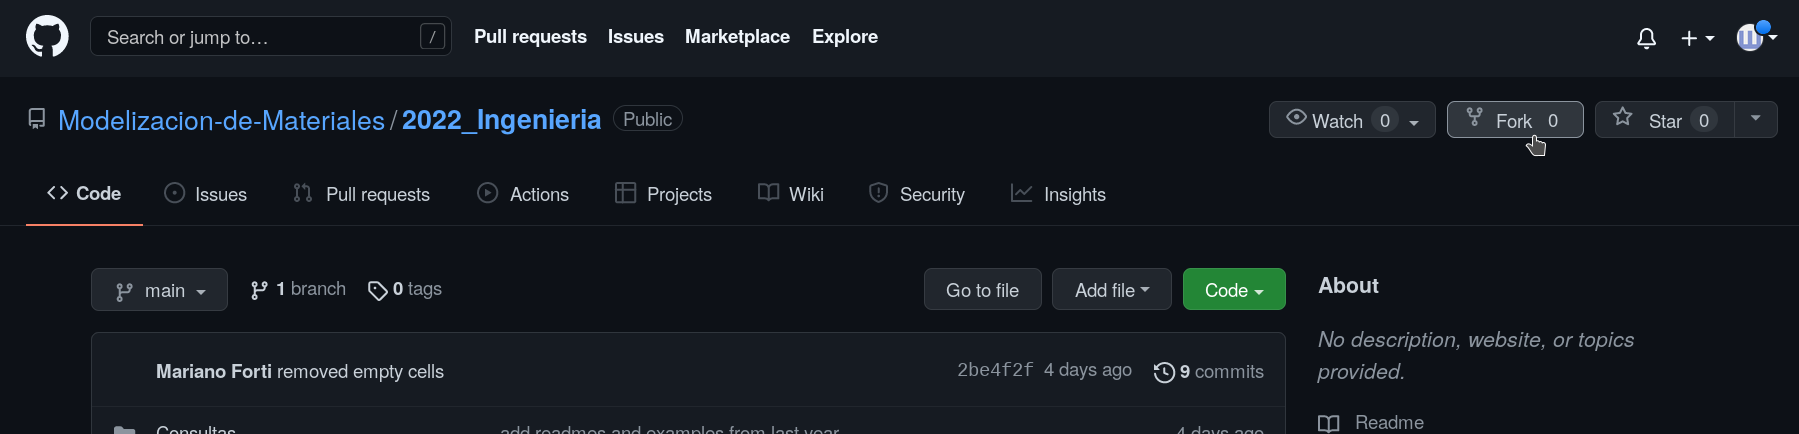
\includegraphics[width=0.9\textwidth]{Screenshots/MakeFork.png}

\end{frame}

\begin{frame}<presentation>[label=FrameCarpetaConsultas]
  \frametitle{Carpeta de Concultas}

  Una vez hecho el for, usted tiene su propia copia del repositorio. EN la misma, genere una carpeta de consutlas.

  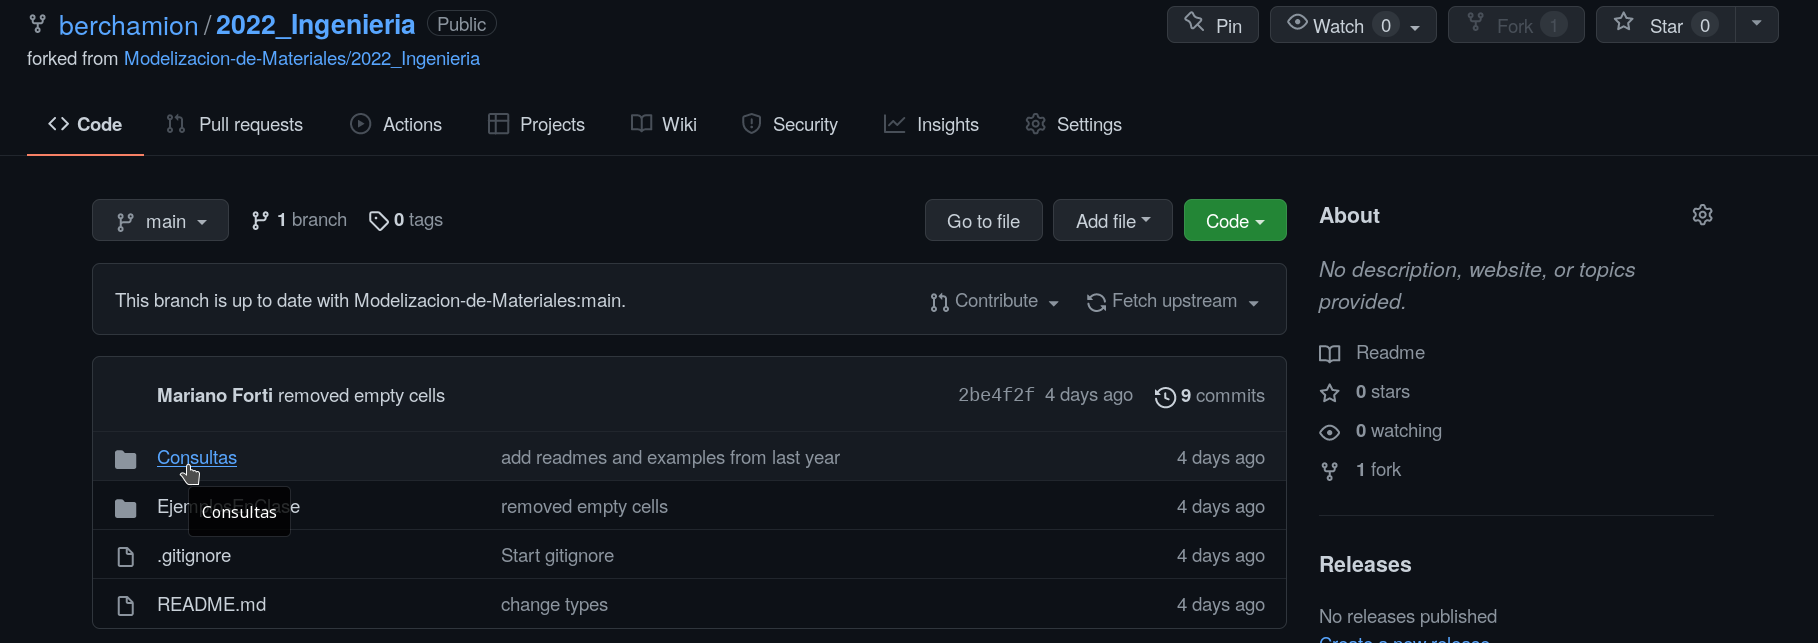
\includegraphics[width=0.5\textwidth]{Screenshots/CarpetaConsultas.png}

\end{frame}

\begin{frame}<presentation>[label=FrameCrearNuevaCarpeta]
  \frametitle{Cree Una carpeta con su nombre}
  \begin{columns}
    \column{0.5\textwidth}
      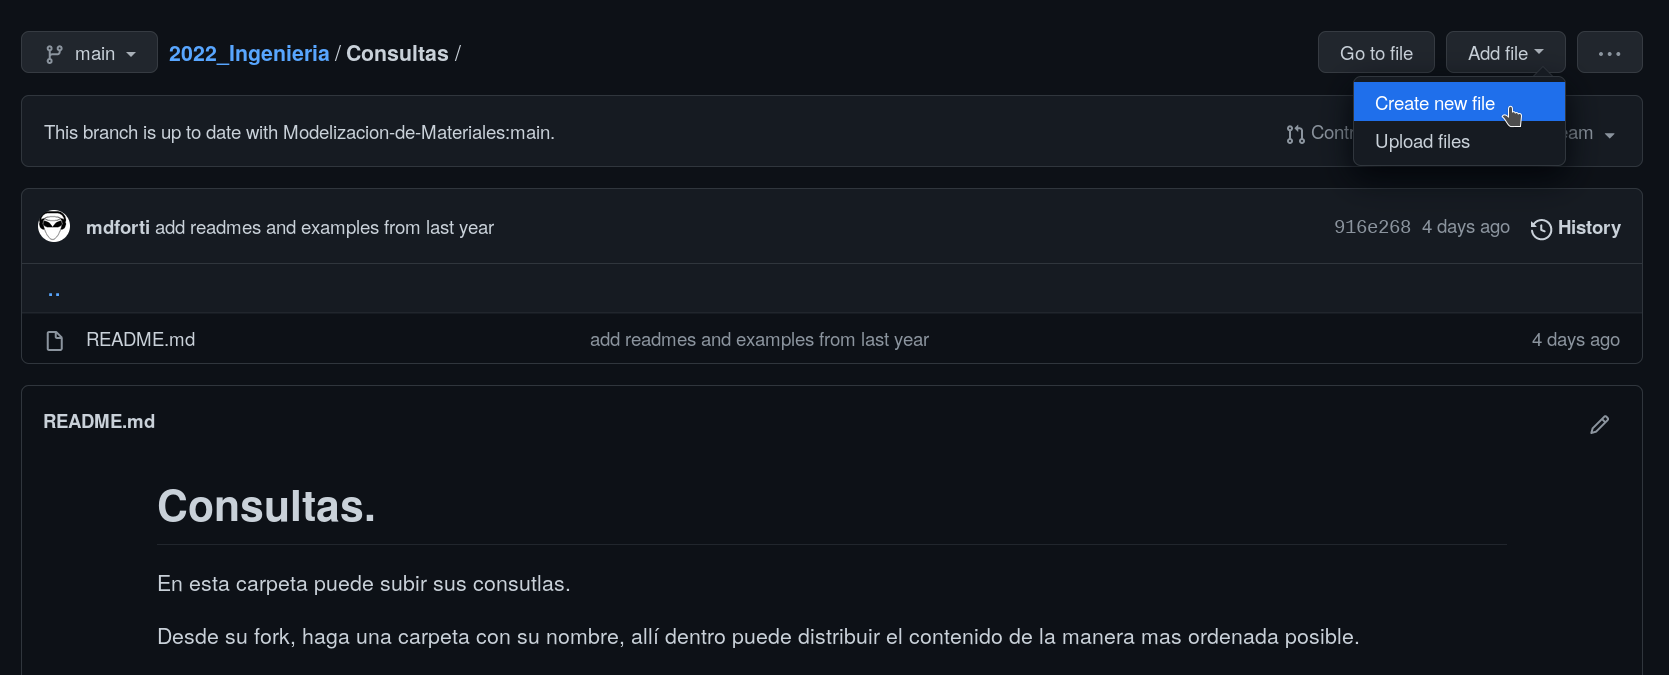
\includegraphics[width=\textwidth]{Screenshots/AddFile_NewFile.png}
      
      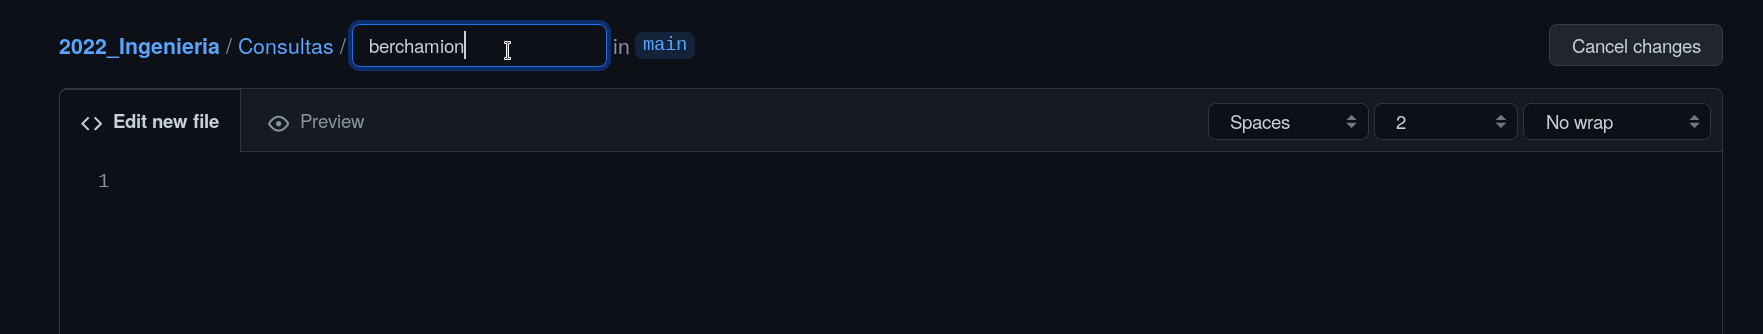
\includegraphics[width=\textwidth]{Screenshots/IngreseSuNombredeCarpeta.png}

      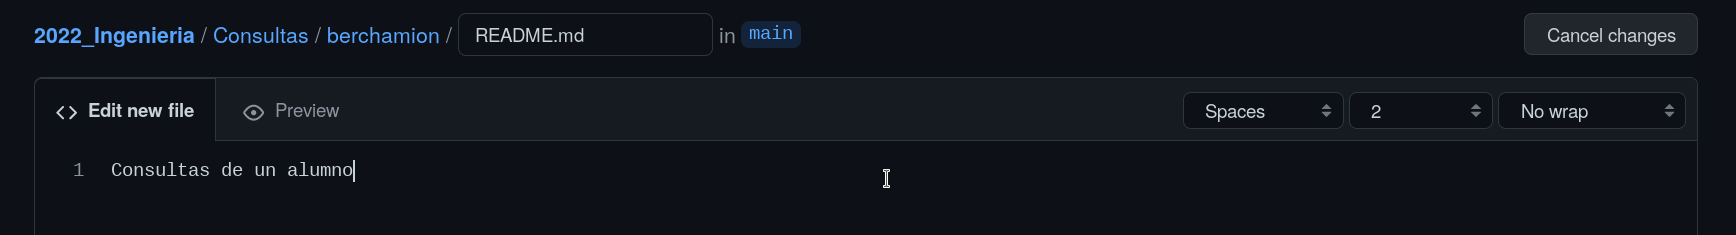
\includegraphics[width=\textwidth]{Screenshots/Readme.png}

      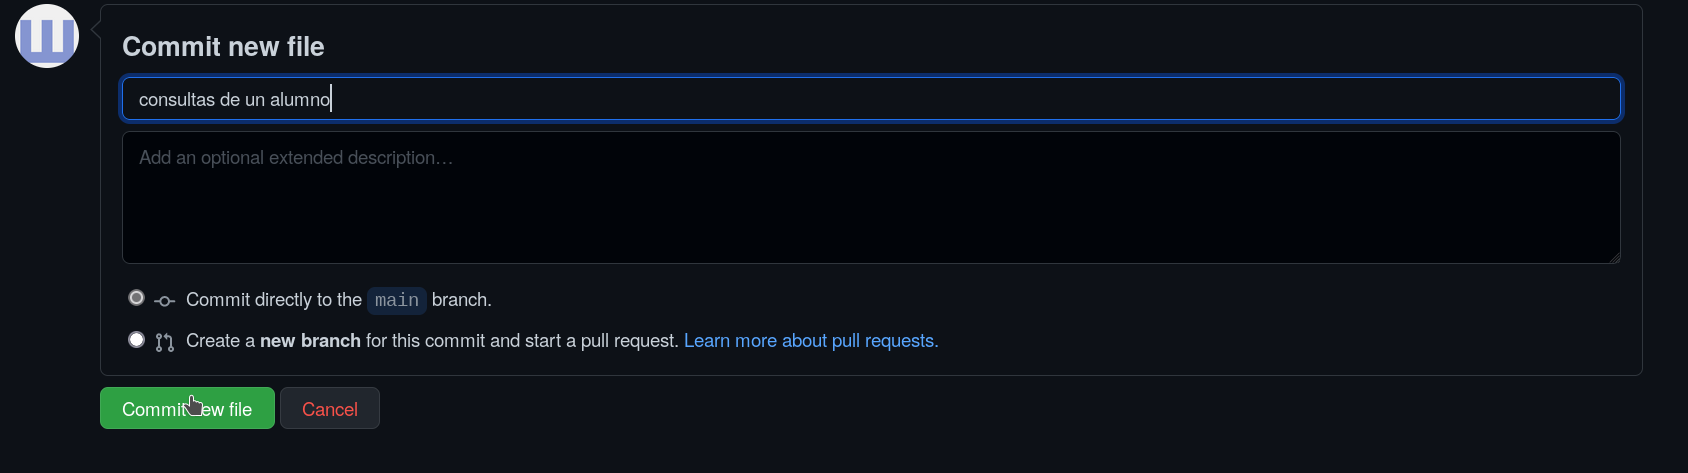
\includegraphics[width=\textwidth]{Screenshots/ScrollComment.png}

    \column{0.5\textwidth}
    \begin{itemize}
      \item Add Files $\quad \rightarrow \quad$  Create new file files
      \item en el cuadro de texto ingrese el nombre de la carpeta terminando con la barra hacia la derecha '/' ,
	la barra es lo que crea la carpeta!
      \item cree un archivo \texttt{README} escrbiendo el nombre luego de la barra con un contenido mínimo
      \item Scroll hacia abajo , ingrese un mínimo comentario explicativo 
      \item confirme los cambios haciendo click en \texttt{commit}
    \end{itemize}
  \end{columns}

\end{frame}

\begin{frame}<presentation>[label=Frame Pull]
  \frametitle{Fetch upstream}

  es una operación para actualizar nuestro repositorio con los últimos cambios en el repositorio de origen (\texttt{upstream} ). 
  Presione en \texttt{Fetch Upstream} y confirme la operación.

  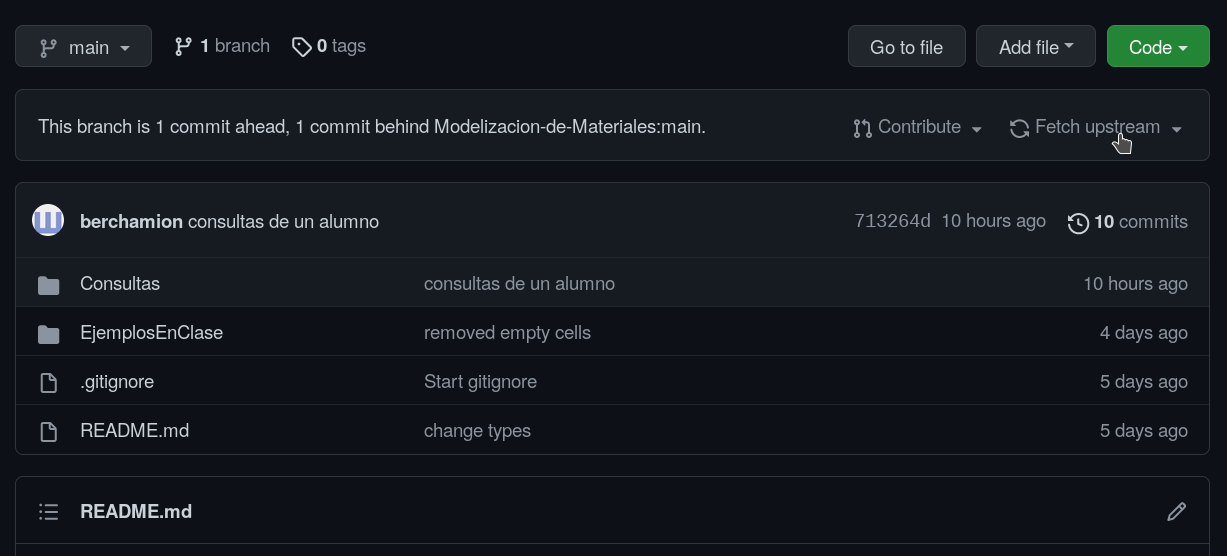
\includegraphics[width=0.4\textwidth]{Screenshots/FetchUpstream.png}
  \quad
  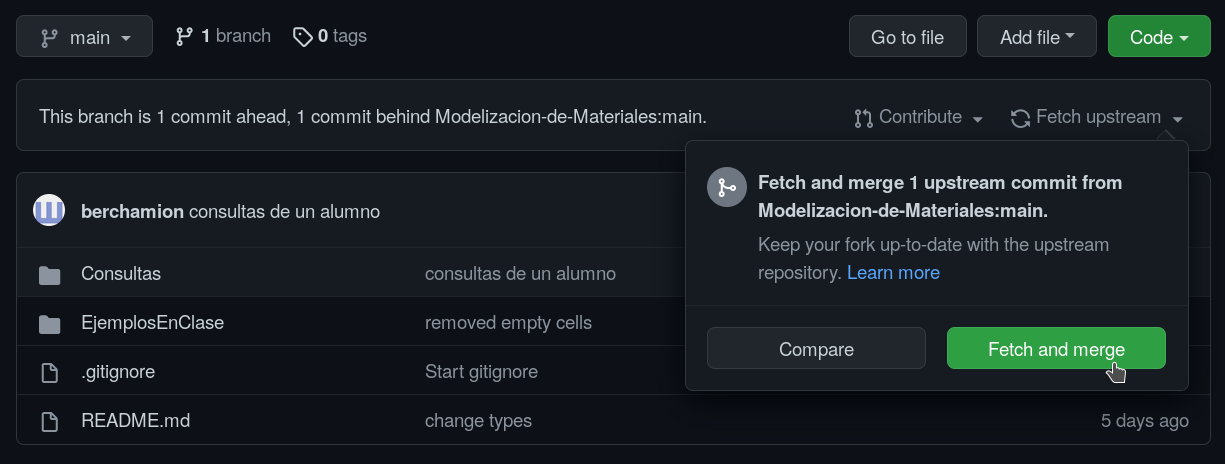
\includegraphics[width=0.4\textwidth]{Screenshots/FetchAndMerge.png}

\end{frame}
\begin{frame}<presentation>[label=FramePullRequest]
  \frametitle{Pull Request}
  \small
  \only<1>{
  Es un procedimiento que permite aplicar los cambios de un repositorio en otro. El dueño del repositorio A le avisa al dueño del repositorio B que 
  tiene nuevos cambios en A que quiere aplicar en B. }
\begin{columns}
  \column{0.5\textwidth}
  \only<2> { 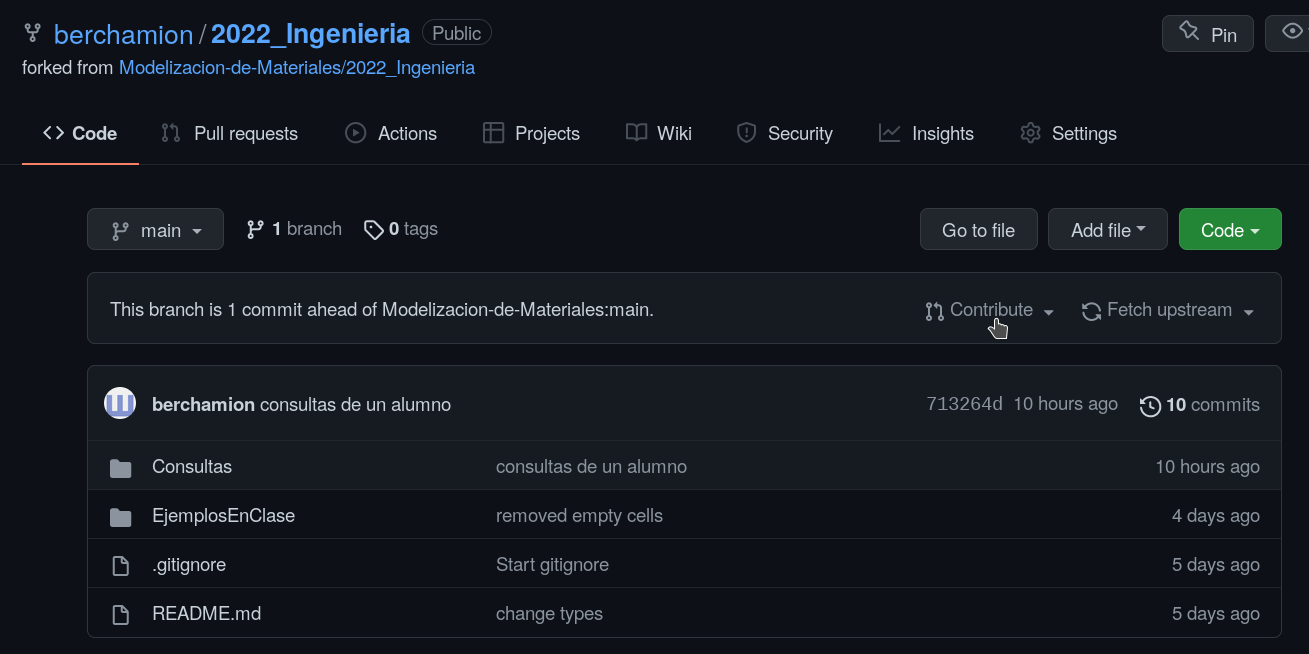
\includegraphics[width=\textwidth]{Screenshots/Contribute.png} }
  \only<2>{ 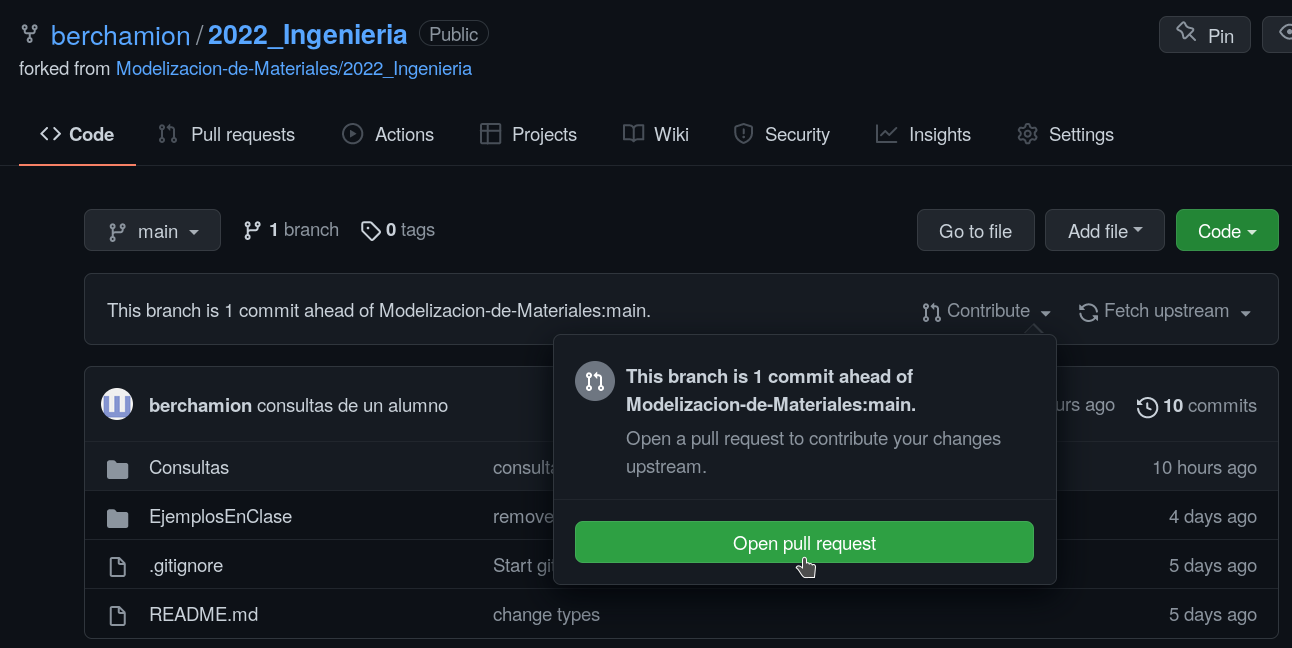
\includegraphics[width=\textwidth]{Screenshots/PulRequest.png}}
  \only<3>{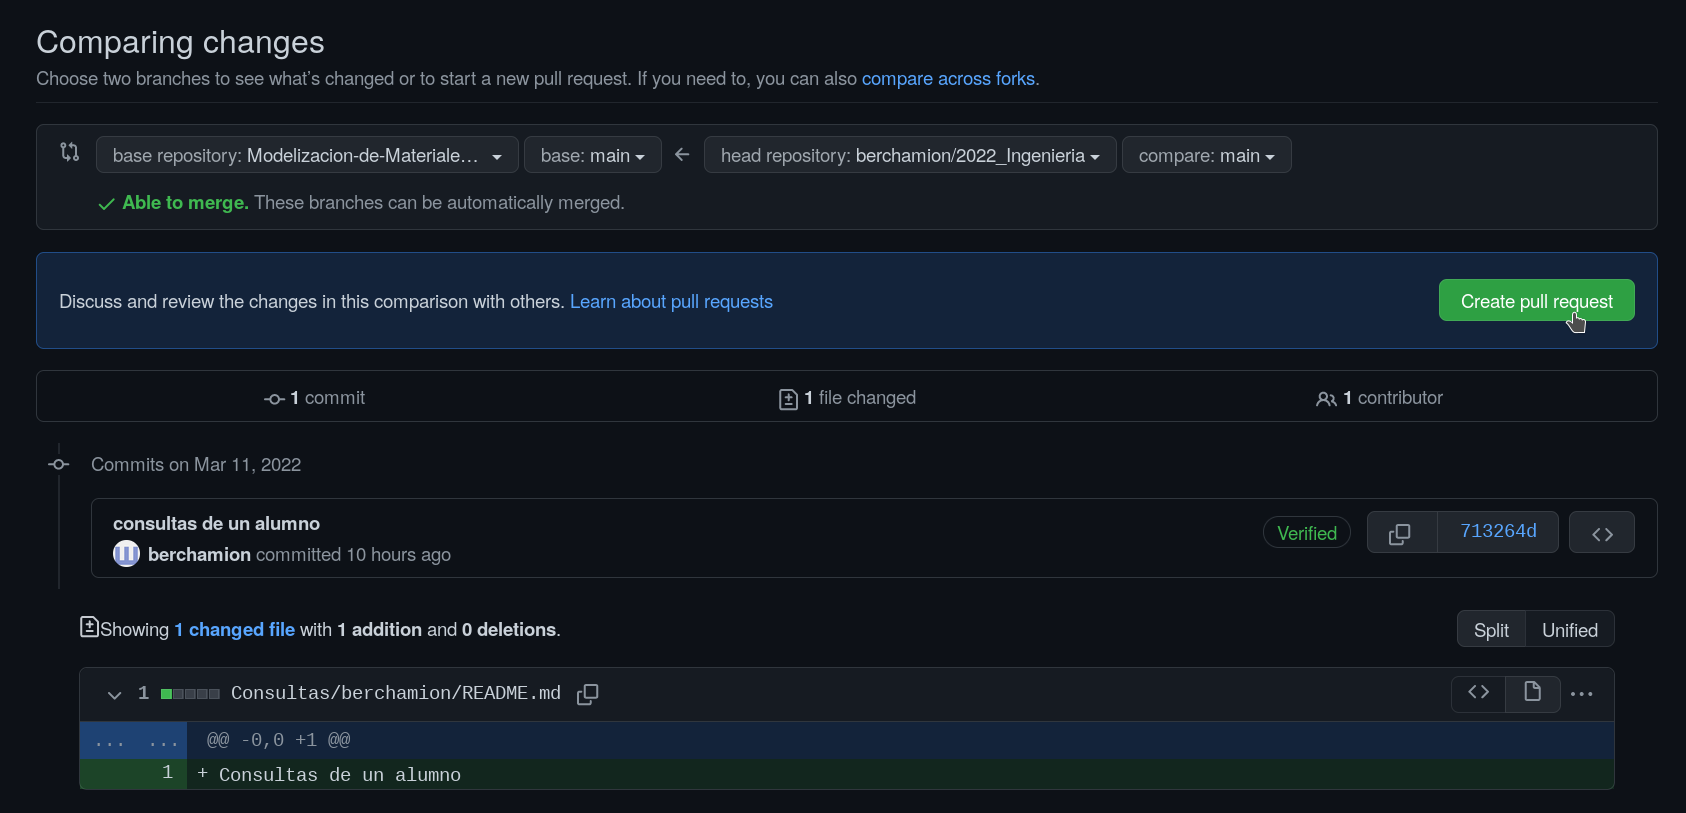
\includegraphics[width=\textwidth]{Screenshots/CheckAndConfirmMerge.png}}
  \only<4> { 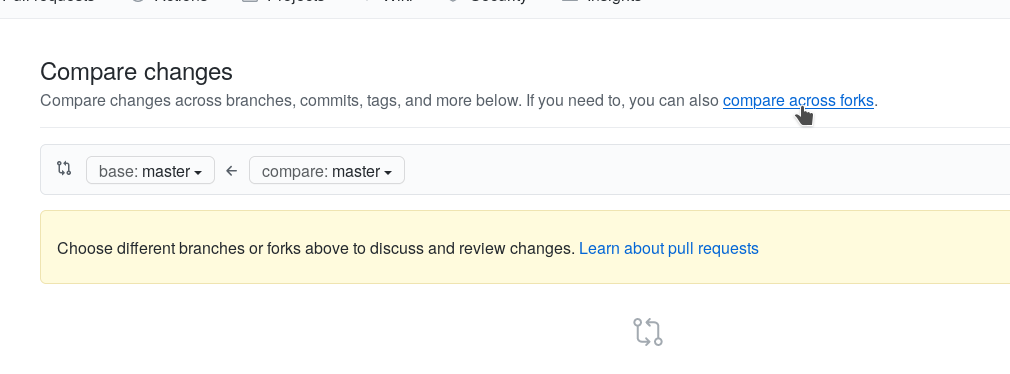
\includegraphics[width=\textwidth]{Screenshots/CompareAcrossForks.png} }
  \column{0.5\textwidth}
  \only<2>{ Desde la pagina inicial de su repositorio ingresar ena  \emph{Contribute} o bien en  \emph{pull request} desde la tira de opciones superior y luego en \emph{ new pull request}. }
  \only<3>{haga un pull request para iniciar su carpeta de consultas en el repositorio de la materia. Preste atención a los campos de \emph{base} y \emph{target}, que correspondan al origien y destino del pull request.}
  \only<4>{  Para poder intercambiar con otros forks del mismo repositorio, haga click en \emph{ comparar a traves de forks } }
\end{columns}

\end{frame}

\begin{frame}<presentation>[label=FrameHeadBase]
  \frametitle{Dirección de Pull Request}

  \only<1>{
  en este paso se elige la dirección en la que se van a aplicar los cambios. preste atención a la flecha entre los 
  menú desplegables. Si quiere forzar a aplicar los ultimos cambios desde el repositorio de la materia, elija 
  las opciones correctas para \texttt{base}(destino)  y \texttt{head repository} (origen). 
}
  \only<2> { Si quiere aplicar los últimos cambios de su repositorio en el de la materia (enviar consultas y entregas) 
  elija \texttt{su\_usuario/Modelizaion-2021-Ingenieria} como \emph{ head} y \texttt{Modelizacion-de-Materiales/Modelizaion-2021-Ingenieria} 
  como \emph{base} }



  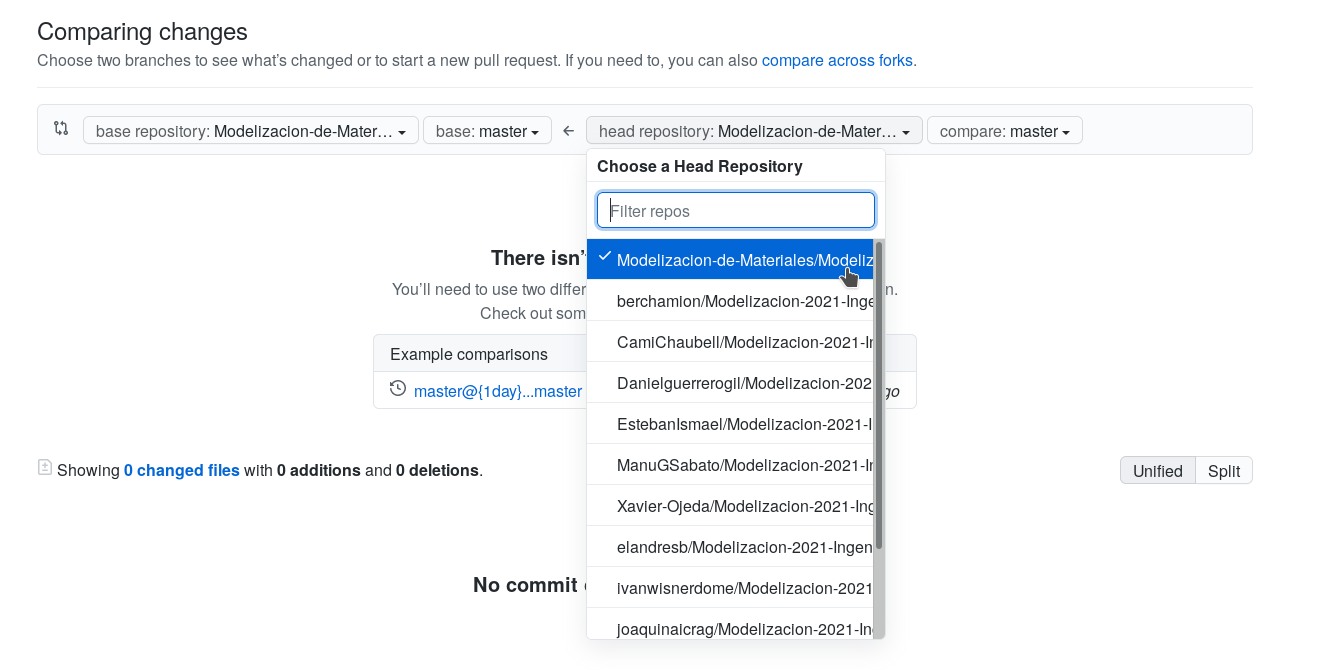
\includegraphics[width=\textwidth]{Screenshots/ToDownload-ChooseHeadMateria.png}

\end{frame}


\begin{frame}<presentation>[label=FrameOptionsChosen]
  \frametitle{Confirme}


  

  \only<1>{
    Confirme la elección para base y head y cree el \emph{pull request} 

  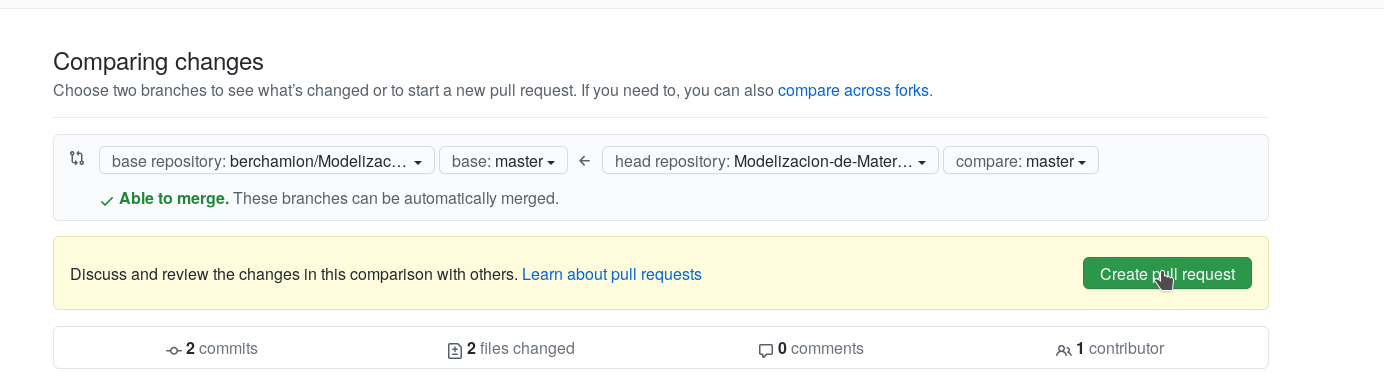
\includegraphics[width=\textwidth]{Screenshots/CreatePullRequest-HeadandBaseChosen.png}
}

  \only<2>{
    comente sobre el contenido de los cambios que se aplicarán, y confirme

    \center

    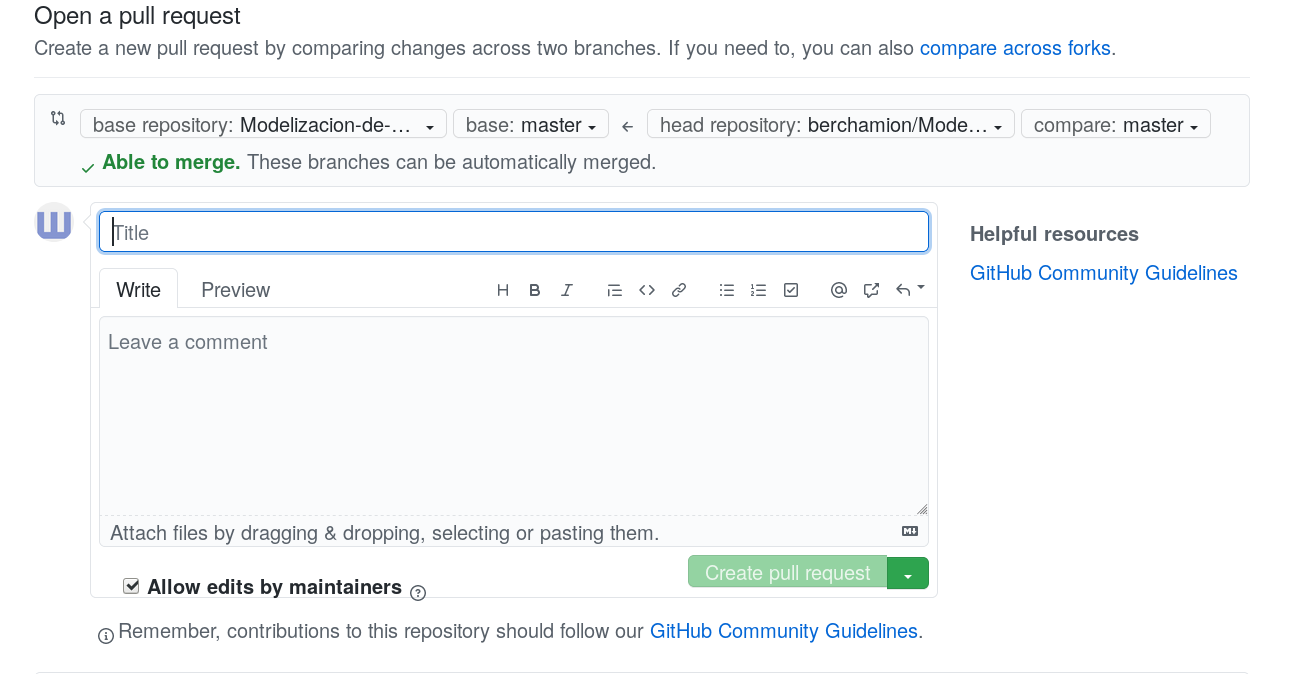
\includegraphics[width=0.5\textwidth]{Screenshots/CommentPullRequest.png}
  }

  \only<3> { si el repsitorio \emph{ base } es el suyo , usted mismo deberá 
  aceptar el \emph{ PR } para aplicar los cambios 
 \center 
  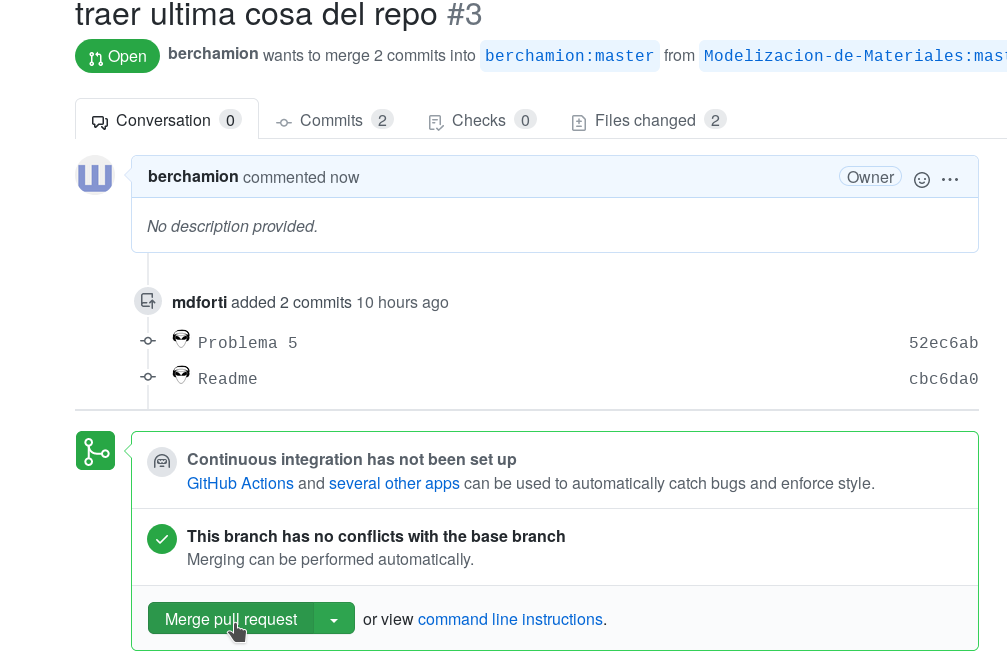
\includegraphics[width=0.5\textwidth]{Screenshots/ConfirmMergeRequest.png}
  }

\end{frame}

\section{ Bajar un único archivo }

\begin{frame}<presentation>[label=FrameDownload]
  \frametitle{Bajar un archivo}

\only<1>{
\begin{itemize}

    \item en el repositorio donde se encuentra el archivo, navege hasta el mismo.

    \item abra el mismo haciedo click sobre el nombre.

    \item note que puede visualizar los JupyterNotebooks y pdf's

    \item busque el botón \emph{raw}

\end{itemize}
} 

\only<2> { 
Se abrirá una pestaña del navegador con el texto plano del archivo. simplemente presione en su teclad:
  \emph{Ctrl + S} y elija la carpeta donde quiere guardarlo.
}

\center 
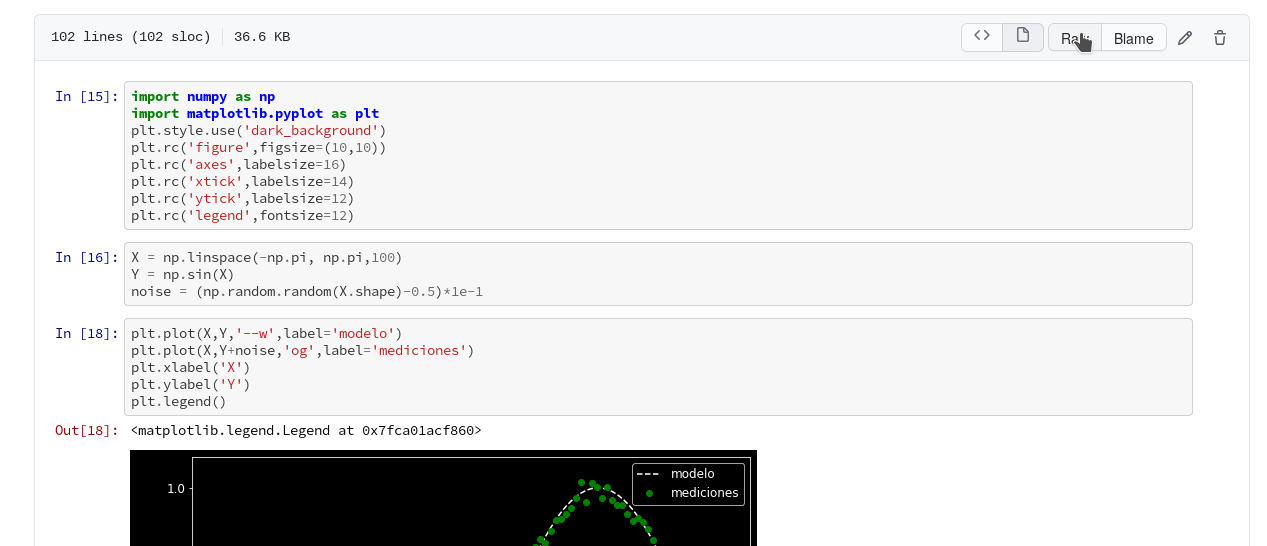
\includegraphics[width=\textwidth]{Screenshots/PressRaw.png}

\end{frame}

\end{document}
